\begin{frame}
\frametitle{Resultados de Regresión Agrupada}

  Regresión Agrupada: Hacemos regresión lineal sobre todos los datos, independientemente de su origen.

  \begin{enumerate}
    \item Para $\fwentrainment{AB}^{(1)}$ no hubo casi resultados significativos
    \item Para $\fwentrainment{AB}^{(2)}$ hubo resultados significativos, pero pocos
  \end{enumerate}

  Para analizar mejor los resultados y eliminar las variables no medidas, efectuamos un análisis de Efectos Fijos.
\end{frame}

\begin{frame}
\frametitle{Regresión Lineal con Efectos Fijos}

  \begin{columns}
    \column{0.40\textwidth}
    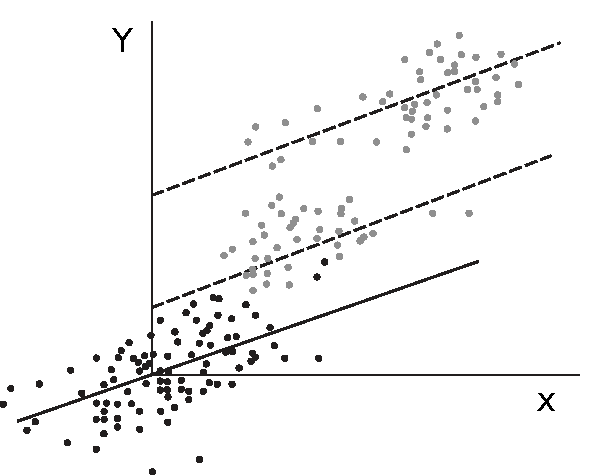
\includegraphics[width=\textwidth]{images/fixed_effects_example.pdf}
    \column{0.60\textwidth}
    \begin{itemize}
      \item Modelo agrupado: niega la posibilidad de heterogeneidad por cada sujeto
      \item Modelo efectos fijos: heterogeneidad no observada constante en el tiempo para cada sujeto.
      \item Varias formas equivalentes de calcularlo: Dummy Variable, Within Group.
      \item En nuestro caso: un sujeto es un hablante dentro de una sesión particular.
    \end{itemize}
  \end{columns}
\end{frame}


\begin{frame}
\frametitle{Regresión Lineal con Efectos Fijos}
\framesubtitle{Resultados}

\begin{table}
  \begin{figure}[ht]
\centering
% psl is "Positive Slope"
\newcommand{\psl} { $+$ }
% nsl stands for "Negative SLope"
\newcommand{\nsl} { $-$ }


\begin{tabular}{| c | c | c | c | c | c |}
  \hline
 & ENG\_MAX & ENG\_MEAN & F0\_MEAN & F0\_MAX & NOISERATIO  \\
  \hline
contributes  &      &  & \psl &  & \psl \\ \hline
  clear     & \psl &  & \psl &  & \psl \\ \hline
  engaged    &      &  & \psl &  &      \\ \hline
  planning   &      &  &      &  &      \\ \hline
  encourages &      &  &      &  &      \\ \hline
  difficult  & \nsl &  &      &  &      \\ \hline
  bored      &      &  & \nsl &  &      \\ \hline
  dislikes   &      &  &      &  &      \\ \hline
   \hline
\end{tabular}

\adjustbox{max width=\textwidth}{
\begin{tabular}{| c | c | c | c | c | c | c |}
  \hline
& PHON\_AVG & PHON\_COUNT & SHIMMER & SYL\_AVG & SYL\_COUNT & VCD2TOT \\
  \hline
contributes  &      &  &  &  &      &  \\ \hline
  clear     & \psl &  &  &  & \psl &  \\ \hline
  engaged    &      &  &  &  &      &  \\ \hline
  planning   &      &  &  &  &      &  \\ \hline
  encourages &      &  &  &  &      &  \\ \hline
  difficult  &      &  &  &  &      &  \\ \hline
  bored      &      &  &  &  &      &  \\ \hline
  dislikes   &      &  &  &  &      &  \\ \hline
  \hline
\end{tabular}
}

\caption{Tabla que representa los resultados significantes del experimento. En una de las entradas, tenemos los nombres abreviados de las variables sociales, y en la otra las variables a/p. El símbolo \psl representa valor significante y positivo de la pendiente de la regresión de efectos fijos, mientras que \nsl representa significante y negativo }

\label{sign_table}

\end{figure}

\end{table}

Tabla que resume los resultados significativos del análisis con efectos fijos. \psl indica un valor positivo con significancia $p < 0.10$,  \ppsl con $p < 0.05$  y \pppsl con $p < 0.01$. Análogamente para los valores negativos.

\end{frame}


\begin{frame}
\frametitle{Regresión Lineal con Efectos Fijos}
\framesubtitle{Resultados}
\begin{enumerate}
  \item Casi todas las variables \ap poseen al menos un valor significativo de $\estslope$, destacándose \ENGMEAN, \NOISETOHARMONICS y \FOMEAN.
  \item Las variables sociales positivas se relacionan de manera positiva con la métrica de mimetización, en aquellos casos significantes.
  \item Análogamente ocurre con las variables de connotación negativa, aunque de manera menos clara.
  \item La métrica se comporta de manera consistente a medidas de mimetización acústico-prosódicas desarrolladas en otros trabajos, como en Gravano et al (2015) utilizando patrones entonacionales. \footnote{Agustin Gravano, Stefan Benus, Rivka Levitan, and Julia Hirschberg. Backward mimicry and forward influence in prosodic contour choice in standard american english 2015.}
\end{enumerate}
\end{frame}
